
\subsection{Bonus KNN: Cost-sensitive Classification}
Kelas positif menunjukkan pemesanan batal. False positive (FP) berarti pemesanan
diprediksi batal, tetapi tamu tetap datang. Penjualan ulang kamar tersebut dapat
menimbulkan overbooking. Sesuai spesifikasi bonus, biaya relatif ditetapkan
$C_{FP}=2$ dan $C_{FN}=1$, sehingga objektif evaluasi adalah
$L=2FP+FN$.

KNN menggunakan $k=21$, Manhattan, distance weighting, dan bobot kategori 1.
Split validasi mengikuti kelompok (seed 42; 5.475 baris). Preprocessing dipelajari
hanya dari subset train. Skor validasi dihitung sekali, lalu threshold diuji dari
0 sampai 1 dengan langkah 0,01, ditambah 0,5 dan $2/3$. Prediksi batal
diberikan jika skor lebih besar daripada threshold. Biaya seri dipecahkan
dengan macro F1 terbesar, lalu threshold terkecil.

Jika $p$ adalah probabilitas batal terkalibrasi, biaya prediksi batal adalah
$2(1-p)$ dan biaya prediksi tidak batal adalah $p$. Maka batas teoritisnya
$p>2/3$. Skor voting KNN belum tentu terkalibrasi, sehingga batas ini digunakan
sebagai pembanding terhadap pemilihan empiris.

\begin{center}
\begin{tabular}{lrrrrr}
\hline
Strategi & Threshold & FP & FN & Biaya & Macro F1 \\
\hline
Baseline & 0.50 & 290 & 455 & 1035 & 0.841689 \\
Teoretis & $2/3$ & 108 & 746 & 962 & 0.801879 \\
Minimum validasi & 0.60 & 158 & 623 & 939 & 0.825069 \\
\hline
\end{tabular}
\end{center}

Threshold 0.60 menurunkan biaya dari 1035 menjadi 939,
atau 9.28\%. FP berkurang tetapi FN bertambah, dan macro F1 turun.
Keputusan ini menunjukkan trade-off ketika FP lebih mahal. Threshold bonus
dipilih untuk objektif biaya, sedangkan konfigurasi submission utama tetap
mengikuti eksperimen macro F1.

\begin{center}
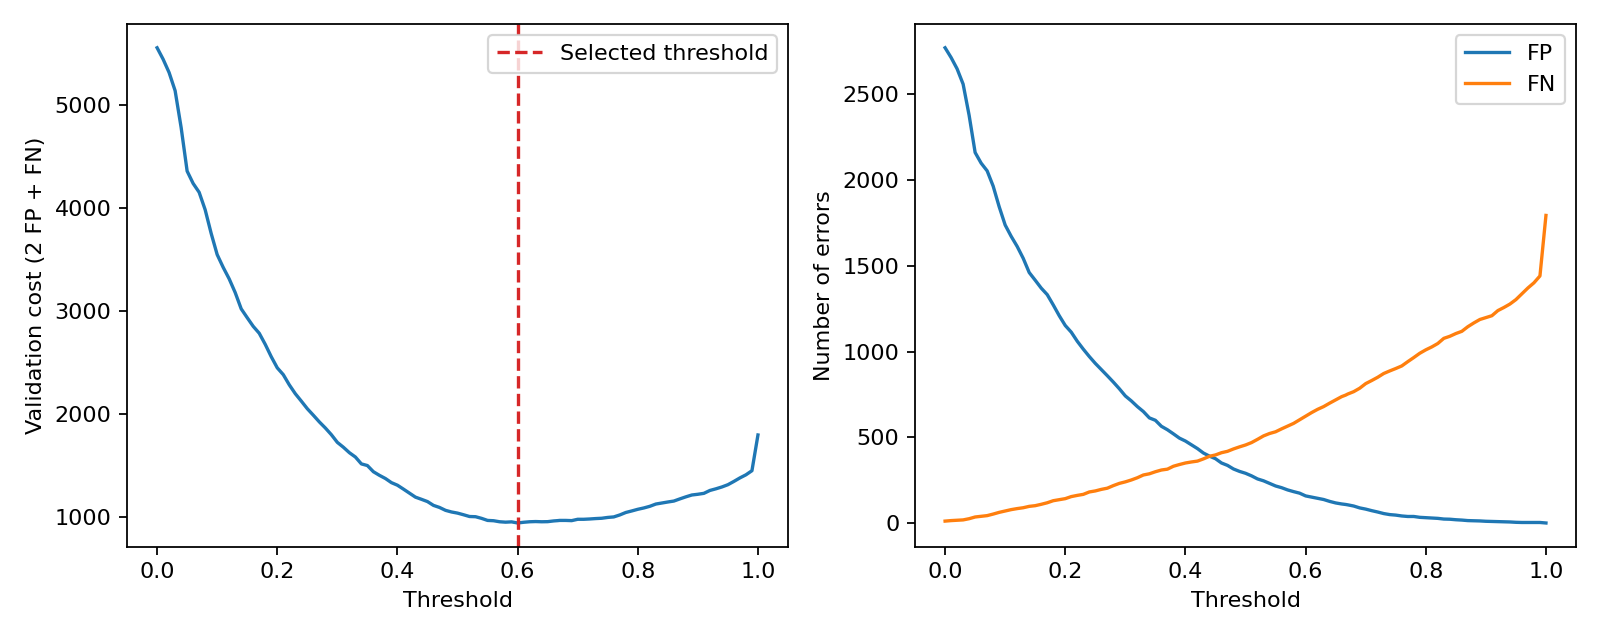
\includegraphics[width=0.95\textwidth]{../../output/knn_cost_sensitive.png}
\end{center}

Pemilihan dan pelaporan threshold dilakukan pada validasi yang sama, sehingga
penurunan biaya dapat optimistis. Angka tersebut merupakan minimum di antara
kandidat pada split ini. Evaluasi independen diperlukan untuk mengukur
generalisasi. Test tanpa label tidak digunakan untuk pemilihan threshold.
Sumber asumsi biaya adalah spesifikasi Tugas Besar 2 IF3170 2026/2027,
bagian Bonus poin 7. Batas teoritis diturunkan langsung dari biaya harapan.
